% CS631 Advanced Programming in the UNIX Environment
% Author: Jan Schaumann <jschauma@netmeister.org>
% $Id: slides.tex,v 1.2 2005/11/01 16:41:35 jschauma Exp $
\special{! TeXDict begin /landplus90{true}store end }

\documentclass[xga]{xdvislides}
\usepackage[landscape]{geometry}
\usepackage{graphics}
\usepackage{graphicx}
\usepackage{colordvi}

\begin{document}
\setfontphv

%%% Headers and footers
\lhead{\slidetitle}
\chead{CS631 - Advanced Programming in the UNIX Environment}
\rhead{Slide \thepage}
\lfoot{\Gray{Lecture 09: D\ae mon processes, System Logging, Shared Libraries }}
\cfoot{\relax}
\rfoot{\Gray{\today}}

\vspace*{\fill}
\begin{center}
	\Hugesize
		CS631 - Advanced Programming in the UNIX Environment\\
		-- \\
		HTTP, D\ae mon processes, System Logging, Shared Libraries\\
	\hspace*{5mm}\blueline\\ [1em]
	\Normalsize
		Department of Computer Science\\
		Stevens Institute of Technology\\
		Jan Schaumann\\
		\verb+jschauma@stevens.edu+\\
		\verb+http://www.cs.stevens.edu/~jschauma/631/+
\end{center}
\vspace*{\fill}

\subsection{HTTP}
\vspace{.5in}
\begin{center}
	\verb+http://www.cs.stevens.edu/~jschauma/631/f13-final-project.html+ \\
	\vspace{.5in}
	\Huge
	Hypertext Transfer Protocol
	\\
	\vspace{.5in}
	RFC2616
\end{center}
\Normalsize

\subsection{HTTP}
\vspace{.5in}
\begin{center}
	\Huge
	HTTP is a request/response protocol.
\end{center}
\Normalsize

\subsection{The Hypertext Transfer Protocol}
HTTP is a request/response protocol:
\begin{enumerate}
	\item client sends a request to the server
	\item server responds
\end{enumerate}

\subsection{The Hypertext Transfer Protocol}
HTTP is a request/response protocol:
\begin{enumerate}
	\item client sends a request to the server
		\begin{itemize}
			\item request method
			\item URI
			\item protocol version
			\item request modifiers
			\item client information
		\end{itemize}
	\item server responds
\end{enumerate}

\subsection{HTTP: A client request}
\vspace*{.5in}
\\
\Hugesize
\begin{center}
\begin{verbatim}
$ telnet www.google.com 80
Trying 2607:f8b0:400c:c02::93...
Connected to www.google.com.
Escape character is '^]'.
GET / HTTP/1.0

\end{verbatim}
\end{center}
\Normalsize
\vspace*{\fill}


\subsection{The Hypertext Transfer Protocol}
HTTP is a request/response protocol:
\begin{enumerate}
	\item client sends a request to the server
		\begin{itemize}
			\item request method
			\item URI
			\item protocol version
			\item request modifiers
			\item client information
		\end{itemize}
	\item server responds
		\begin{itemize}
			\item status line (including success or error code)
			\item server information
			\item entity metainformation
			\item content
		\end{itemize}
\end{enumerate}

\subsection{HTTP: a server response}
%\newcommand{\smallish}{\fontsize{18}{18}\selectfont}
%\smallish
\begin{verbatim}
HTTP/1.0 200 OK
Date: Mon, 22 Oct 2012 03:08:18 GMT
Content-Type: text/html; charset=ISO-8859-1
Server: gws

<!doctype html><html itemscope="itemscope"
itemtype="http://schema.org/WebPage"><head><meta content="Search the
world's information, including webpages, images, videos and more. Google
has many special features to help you find exactly what you're looking
for." name="description"><meta content="noodp" name="robots"><meta
itemprop="image"
content="/images/google_favicon_128.png"><title>Google</title><script>
window.google={kEI:"oriEUNmMGMX50gH6kYGwBw",getEI:function(a){var
b;while(a&&!(a.getAttribute&&(b=a.getAttribute("eid"))))a=a.parentNode;return
b||google.kEI},https:function(){return
window.location.protocol=="https:"},kEXPI:"25657,30316,39523,39977,40362
\end{verbatim}
%\Normalsize

\subsection{The Hypertext Transfer Protocol}
Server status codes:
\begin{itemize}
	\item {\bf 1xx} -- Informational; Request received, continuing process
	\item {\bf 2xx} -- Success; The action was successfully received,
        understood, and accepted
	\item {\bf 3xx} -- Redirection; Further action must be taken in order to
        complete the request
	\item {\bf 4xx} -- Client Error; The request contains bad syntax or
		cannot be fulfilled
	\item {\bf 5xx} -- Server Error; The server failed to fulfill an
		apparently valid request
\end{itemize}

\subsection{HTTP: A client request}
\newcommand{\smallish}{\fontsize{16}{16}\selectfont}
\smallish
\begin{center}
\begin{verbatim}
$ telnet www.cs.stevens.edu 80
Trying 155.246.89.84...
Connected to tarantula.srcit.stevens-tech.edu.
Escape character is '^]'.
GET / HTTP/1.0

HTTP/1.1 200 OK
Date: Mon, 04 Apr 2011 02:16:14 GMT
Server: Apache/2.2.9 (Debian) DAV/2 SVN/1.5.1 PHP/5.2.6-1+lenny9 with Suhosin-Patch mod_ssl/2.2.9 OpenSSL/0.9.8o
Last-Modified: Wed, 17 Nov 2010 19:25:54 GMT
Content-Type: text/html

<!DOCTYPE HTML PUBLIC "-//W3C//DTD HTML 4.0 Transitional//EN">
<html>
<head>
<title>SRCIT wiki page</title>
<meta http-equiv="REFRESH"
content="0;url=http://www.srcit.stevens.edu/wiki"></HEAD>
<BODY>
</BODY>
</HTML>
\end{verbatim}
\end{center}
\Normalsize

\subsection{HTTP - more than just text}
HTTP is a {\em Transfer Protocol} -- serving {\em data}, not any specific
text format.

\begin{itemize}
	\item {\tt Accept-Encoding} client header can specify different formats
		such as {\em gzip}, {\em Shared Dictionary Compression over HTTP (SDCH)} etc.
	\item corresponding server headers: {\tt Content-Type} and
		{\tt Content-Encoding}
\end{itemize}
\begin{center}
	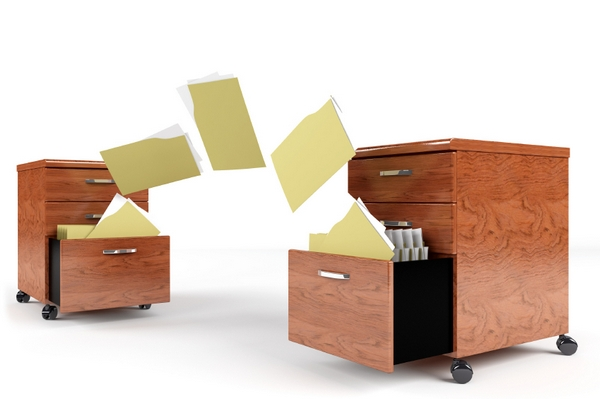
\includegraphics[scale=0.6,angle=-90]{pics/datatransfer.eps}
\end{center}

\subsection{HTTP - more than just static data}
HTTP is a {\em Transfer Protocol} -- what is transferred need not be
static; resources may generate different data to return based on many
variables.

\begin{itemize}
	\item CGI -- resource is {\em executed}, needs to generate
		appropriate response headers
	\item server-side scripting (ASP, PHP, Perl, ...)
	\item client-side scripting (JavaScript/ECMAScript/JScript,...)
	\item applications based on HTTP, using:
		\begin{itemize}
			\item AJAX
			\item RESTful services
			\item JSON, XML, YAML to represent state and
				abstract information
		\end{itemize}
\end{itemize}

\subsection{Writing a {\em simple} HTTP server}
\begin{itemize}
	\item parse command-line options, initialize world, ...
	\item open socket
	\item run as a d\ae mon, loop forever
		\begin{itemize}
			\item accept connection
			\item fork child to handle request
		\end{itemize}
	\item upon {\tt SIGHUP} re-read configuration, restart
\end{itemize}

\subsection{Writing a {\em simple} HTTP server}
Processing requests consists of:
\begin{itemize}
	\item reading request from socket
	\item parsing request
		\begin{itemize}
			\item valid syntax?
			\item type of request (GET, HEAD, POST)?
			\item determine pathname
				\begin{itemize}
					\item $\sim$ translation
					\item translate relative into absolute pathname
				\end{itemize}
		\end{itemize}
	\item generate server status response
	\item handle request
\end{itemize}

\subsection{Writing a {\em simple} HTTP server}
Processing requests consists of:
\begin{itemize}
	\item handling regular file request
		\begin{itemize}
			\item {\tt stat(2)} file
			\item {\tt open(2)} file
			\item {\tt read(2)} file
			\item {\tt write(2)} to socket
			\item {\tt close(2)} file
			\item terminate connection
			\item exit child handler
		\end{itemize}
	\item handling CGI execution
		\begin{itemize}
			\item setup environment
			\item setup filedescriptors (stdin/stdout)
			\item fork-exec executable
		\end{itemize}
\end{itemize}



\subsection{Client-Server Model}
\begin{itemize}
	\item two categories of of servers
		\begin{enumerate}
			\item iterative
			\item concurrent
		\end{enumerate}
\end{itemize}

\subsection{Client-Server Model}
\begin{itemize}
	\item two categories of of servers
		\begin{enumerate}
			\item iterative
				\begin{enumerate}
					\item wait for client request to arrive
					\item process the client request
					\item send the response back to the client
					\item go back to 1.1
				\end{enumerate}
			\item concurrent
		\end{enumerate}
\end{itemize}

\subsection{Client-Server Model}
\begin{itemize}
	\item two categories of of servers
		\begin{enumerate}
			\item iterative
				\begin{enumerate}
					\item wait for client request to arrive
					\item process the client request
					\item send the response back to the client
					\item go back to 1.1
				\end{enumerate}
			\item concurrent
				\begin{enumerate}
					\item wait for client request to arrive
					\item start a new server to handle this client's request
					\item go back to 2.1
				\end{enumerate}
		\end{enumerate}
\end{itemize}

\subsection{D\ae mon processes}
So... what's a d\ae mon process anyway?
\vfill
\hfill
\includegraphics[scale=0.5]{pics/daemon.eps} \\

\subsection{D\ae mon characteristics}
Commonly, d\ae mon processes are created to offer a specific service.
\\

D\ae mon processes usually
\begin{itemize}
	\item live for a long time
	\item are started at boot time
	\item terminate only during shutdown
	\item have no controlling terminal
\end{itemize}

\vfill
\hfill
\includegraphics[scale=0.5]{pics/daemon.eps} \\

\subsection{D\ae mon characteristics}
The previously listed characteristics have certain implications:
\\

\begin{itemize}
	\item do one thing, and one thing only
	\item no (or only limited) user-interaction possible
	\item consider current working directory
	\item how to create (debugging) output
\end{itemize}

\vfill
\hfill
\includegraphics[scale=0.5]{pics/daemon.eps} \\

\subsection{Writing a d\ae mon}
\begin{itemize}
	\item fork off the parent process
	\item change file mode mask (umask)
	\item create a unique Session ID (SID)
	\item change the current working directory to a safe place
	\item close (or redirect) standard file descriptors
	\item open any logs for writing
	\item enter actual d\ae mon code
\end{itemize}

\vfill
\hfill
\includegraphics[scale=0.5]{pics/daemon.eps} \\

\subsection{Writing a d\ae mon}
\small
\begin{verbatim}
int
daemon(int nochdir, int noclose)
{
        int fd;

        switch (fork()) {
        case -1:
                return (-1);
        case 0:
                break;
        default:
                _exit(0);
        }

        if (setsid() == -1)
                return (-1);

        if (!nochdir)
                (void)chdir("/");

        if (!noclose && (fd = open(_PATH_DEVNULL, O_RDWR, 0)) != -1) {
                (void)dup2(fd, STDIN_FILENO);
                (void)dup2(fd, STDOUT_FILENO);
                (void)dup2(fd, STDERR_FILENO);
                if (fd > STDERR_FILENO)
                        (void)close(fd);
        }
        return (0);
}
\end{verbatim}
\Normalsize

\subsection{D\ae mon conventions}
\begin{itemize}
	\item prevent against multiple instances via a {\em lockfile}
	\item allow for easy determination of PID via a {\em pidfile}
	\item configuration file convention {\tt /etc/{\em name}.conf}
	\item include a system initialization script (for {\tt /etc/rc.d/} or {\tt
		/etc/init.d/})
	\item re-read configuration file upon {\tt SIGHUP}
\end{itemize}

\vfill
\hfill
\includegraphics[scale=0.5]{pics/daemon.eps} \\


\subsection{Logging}

\subsection{A central logging facility}

There are three ways to generate log messages:
\begin{itemize}
	\item via the kernel routine {\tt log(9)}
	\item via the userland routine {\tt syslog(3)}
	\item via UDP messages to port 514
\end{itemize}

\subsection{A central logging facility}
\begin{center}
	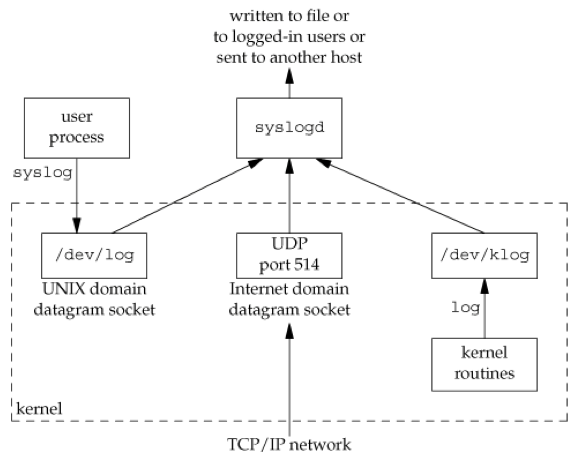
\includegraphics[scale=0.8,angle=-90]{pics/syslog.eps}
\end{center}



\subsection{\tt syslog(3)}
\small
\setlength{\unitlength}{1mm}
\begin{center}
	\begin{picture}(150,22)
		\thinlines
		\put(0,0){\framebox(130,22){}}
		\put(10,17){{\tt \#include <syslog.h>}}
		\put(10,10){{\tt void openlog(const char *{\em ident}, int {\em logopt}, int {\em facility});}}
		\put(10,5){{\tt void syslog(int {\em priority}, const char *{\em message}, ...);}}
	\end{picture}
\end{center}
\Normalsize
{\tt openlog(3)} allows us to set specific options when logging:
\begin{itemize}
	\item prepend {\em ident} to each message
	\item specify logging options ({\tt LOG\_CONS | LOG\_NDELAY | LOG\_PERRO | LOG\_PID})
	\item specify a {\em facility} (such as {\tt LOG\_DAEMON}, {\tt LOG\_MAIL} etc.)
\end{itemize}
\vspace{.5in}
{\tt syslog(3)} writes a message to the system message logger, tagged with
{\em priority}. \\
A {\em priority} is a combination of a {\em facility} (as above) and a {\em level} (such
as {\tt LOG\_DEBUG}, {\tt LOG\_WARNING} or {\tt LOG\_EMERG}).

\subsection{Shared Libraries}
What is a shared library, anyway?

\subsection{Shared Libraries}
What is a shared library, anyway?
\begin{itemize}
	\item contains a set of callable C functions (ie, implementation
		of function prototypes defined in {\tt .h} header files)
	\item code is position-independent (ie, code can be executed anywhere
		in memory)
	\item shared libraries can be loaded/unloaded at execution time or at will
	\item libraries may be {\em static} or {\em dynamic}
\end{itemize}

\subsection{Shared Libraries}
What is a shared library, anyway?
\begin{itemize}
	\item contains a set of callable C functions (ie, implementation
		of function prototypes defined in {\tt .h} header files)
	\item code is position-independent (ie, code can be executed anywhere
		in memory)
	\item shared libraries can be loaded/unloaded at execution time or at will
	\item libraries may be {\em static} or {\em dynamic}
\end{itemize}
\begin{verbatim}
$ man 3 fprintf
$ grep " fprintf" /usr/include/stdio.h
\end{verbatim}


\subsection{Shared Libraries}
How do shared libraries work?
\begin{itemize}
	\item contents of {\em static} libraries are pulled into the
		executable at link time
	\item contents of {\em dynamic} libraries are used to resolve
		symbols at {\bf link time}, but loaded at {\bf execution time} by the
		{\em dynamic linker}
	\item contents of {\em dynamic} libraries may be loaded at {\bf any
		time} via explicit calls to the dynamic linking loader interface
		functions
\end{itemize}

\subsection{Executable and Linkable Format}

{\bf ELF} is a file format for executables, object code, shared libraries
etc.

\begin{center}
	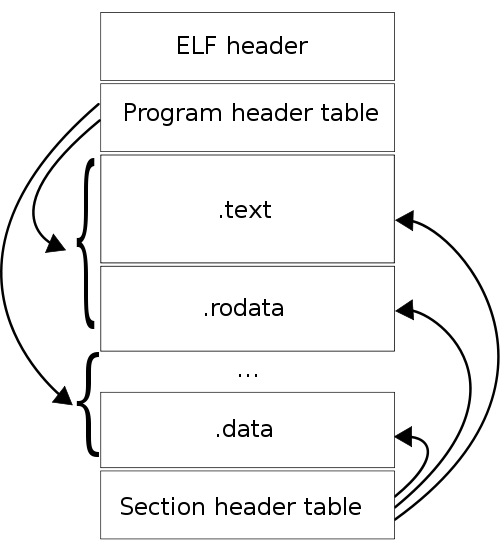
\includegraphics[scale=0.5]{pics/elf.eps}
\end{center}
More details:
\verb+http://www.cs.stevens.edu/~jschauma/631/elf.html+

\verb+http://www.thegeekstuff.com/2012/07/elf-object-file-format/+
\Normalsize


\subsection{Understanding object files}
\begin{verbatim}
$ cc -Wall -c ldtest1.c ldtest2.c main.c
$ readelf -h ldtest1.o
[...]
$ cc *.o
$ readelf -h a.out
[...]
$ ldd a.out
[...]
$ readelf -h /lib/libc.so.6
[...]
$ readelf -s a.out | more
[...]
$ objdump -d -j .text a.out | more
[...]
$ nm -D a.out | more
[...]
$
\end{verbatim}

\subsection{Statically Linked Shared Libraries}
Static libraries:
\begin{itemize}
	\item created by {\tt ar(1)}
	\item usually end in {\tt .a}
	\item contain a symbol table within the archive (see {\tt
		ranlib(1)})
\end{itemize}

\subsection{Statically Linked Shared Libraries}
\begin{verbatim}
$ cc -Wall -c ldtest1.c
$ cc -Wall -c ldtest2.c
$ cc -Wall main.c
[...]
$ cc -Wall main.c ldtest1.o ldtest2.o
$
\end{verbatim}

\subsection{Statically Linked Shared Libraries}
\begin{verbatim}
$ cc -Wall -c ldtest1.c ldtest2.c
$ ar -vq libldtest.a ldtest1.o ldtest2.o
$ ar -t libldtest.a
$ cc -Wall main.c libldtest.a

$ cc -Wall -c main.c
$ cc main.o -L. -lldtest -o a.out.dyn
$ cc -static main.o -L. -lldtest -o a.out.static
$ ls -l a.out.*
$ ldd a.out.*
$ nm a.out.dyn | wc -l
$ nm a.out.static | wc -l
\end{verbatim}

\subsection{Dynamically Linked Shared Libraries}
Explicit loading of shared libraries:
\begin{itemize}
	\item {\tt dlopen(3)} creates a handle for the given library
	\item {\tt dlsym(3)} returns the address of the given symbol
	\item
\end{itemize}

\begin{verbatim}
$ cc -Wall setget.c
$ cc -Wall -rdynamic dlopenex.c -ldl
$ ./a.out
\end{verbatim}

\subsection{Dynamically Linked Shared Libraries}
Dynamic libraries:
\begin{itemize}
	\item created by the compiler/linker (ie multiple steps)
	\item usually end in {\tt .so}
	\item frequently have multiple levels of symlinks providing
		backwards compatibility / ABI definitions
\end{itemize}

\subsection{Dynamically Linked Shared Libraries}
\begin{verbatim}
$ rm *.o libldtest*
$ cc -Wall -c -fPIC ldtest1.c
$ cc -Wall -c -fPIC ldtest2.c
$ mkdir lib
$ cc -shared -Wl,-soname,libldtest.so.1 -o lib/libldtest.so.1.0 ldtest1.o ldtest2.o
$ ln -s libldtest.so.1.0 lib/libldtest.so.1
$ ln -s libldtest.so.1.0 lib/libldtest.so
$ cc -static -Wall main.o -L./lib -lldtest
[...]
$ cc -Wall main.o -L./lib -lldtest
[...]
$ ./a.out
[...]
$ ldd a.out
[...]
\end{verbatim}

\subsection{Dynamically Linked Shared Libraries}
Wait, what?
\begin{verbatim}
$ export LD_LIBRARY_PATH=${LD_LIBRARY_PATH}:./lib
$ ldd a.out
[...]
$ ./a.out
[...]
$ mkdir lib2
$ cc -Wall -c -fPIC ldtest1.2.c
$ cc -shared -Wl,-soname,libldtest.so.1 -o lib2/libldtest.so.1.0 ldtest1.2.o ldtest2.o
$ ln -s libldtest.so.1.0 lib2/libldtest.so.1
$ ln -s libldtest.so.1.0 lib2/libldtest.so
$ export LD_LIBRARY_PATH=./lib2:$LD_LIBRARY_PATH
$ ldd a.out  # note: no recompiling!
[...]
$ ./a.out
[...]
\end{verbatim}

\subsection{Dynamically Linked Shared Libraries}
Avoiding {\tt LD\_LIBRARY\_PATH}:
\begin{verbatim}
$ cc -Wall main.o -L./lib -lldtest -Wl,-rpath,./lib
$ echo $LD_LIBRARY_PATH
[...]
$ ldd a.out
[...]
$ ./a.out
[...]
$ unset LD_LIBRARY_PATH
$ ldd a.out
[...]
$ ./a.out
[...]
$
\end{verbatim}

\subsection{Dynamically Linked Shared Libraries}
But:
\begin{verbatim}
$ cc -Wall -fPIC -c evil.c
$ cc -shared -Wl,-soname,libldtest.so.1 -o lib3/libldtest.so.1.0 \
        ldtest1.o ldtest2.o evil.o
$ export LD_PRELOAD=./lib3/libldtest.so.1.0
$ ldd a.out
[...]
$ ./a.out
[...]
$
\end{verbatim}

\subsection{Dynamically Linked Shared Libraries}
\begin{verbatim}
$ export LD_DEBUG=help # glibc>=2.1 only
$ ./a.out
[...]
$ LD_DEBUG=all ./a.out
[...]
\end{verbatim}

\subsection{Homework}
Same as last week:

\verb+http://www.cs.stevens.edu/~jschauma/631/f13-hw3.html+

\verb+http://www.cs.stevens.edu/~jschauma/631/f13-final-project.html+

\end{document}
